% =====================================================================================
% The HHL quantum linear-systems algorithm - from linear algebra to a CUDA-Q implementation
% Build:  python make_figures.py   (needs cudaq, numpy, scipy, matplotlib)
%         latexmk -pdf hhl_lecture.tex
% Companion of presentations/qft_source/qft_lecture.tex (same layout and colours).
% =====================================================================================
\documentclass[aspectratio=169,11pt]{beamer}
\usepackage[T1]{fontenc}
\usepackage{lmodern}
\usepackage{amsmath,amssymb}
\usepackage{braket}
\usepackage{graphicx}
\usepackage{booktabs}
\usepackage{array}
\usepackage{tikz}
\usetikzlibrary{arrows.meta,positioning}
\usepackage{quantikz}
\usepackage{listings}
\graphicspath{{figures/}}
% GENERATED by make_figures.py - do not edit
\newcommand{\numpstate}{0.355903}
\newcommand{\numacc}{7086}
\newcommand{\numpshots}{0.3543}
\newcommand{\numrelerr}{1.74\times10^{-15}}
\newcommand{\numfiddef}{1.0000000000}
\newcommand{\numshotmax}{0.0069}
\newcommand{\numstaterr}{0.012}
\newcommand{\numsampledrow}{0.7691, 0.0587, 0.1420, 0.0302}
\newcommand{\numpkfour}{0.2891}
\newcommand{\numpkthree}{0.3147}
\newcommand{\numpkoneofthree}{0.3147}
\newcommand{\numfidtwo}{0.2059}
\newcommand{\numfidthree}{0.9532157640}
\newcommand{\numpthree}{0.3285}
\newcommand{\numidealthree}{0.632716}
\newcommand{\numptwo}{0.4222}
\newcommand{\numcthree}{1.3333}
\newcommand{\numptwobytwo}{0.625000}
\newcommand{\numfidtwobytwo}{1.0000000000}
\newcommand{\numgatesrows}{2 & 5 & 23 & 3 & 21\\3 & 6 & 51 & 7 & 38\\4 & 7 & 111 & 15 & 67\\5 & 8 & 235 & 31 & 120\\6 & 9 & 507 & 63 & 221\\7 & 10 & 1099 & 127 & 418\\}


\definecolor{qblue}{HTML}{2A78D6}
\definecolor{qdark}{HTML}{1C5CAB}
\definecolor{qorange}{HTML}{EB6834}
\definecolor{qaqua}{HTML}{1BAF7A}
\definecolor{qink}{HTML}{0B0B0B}
\definecolor{qgrey}{HTML}{52514E}
\definecolor{qlight}{HTML}{EEF4FC}
\setbeamercolor{structure}{fg=qdark}
\setbeamercolor{frametitle}{fg=qdark}
\setbeamercolor{title}{fg=qdark}
\setbeamercolor{normal text}{fg=qink}
\setbeamercolor{block title}{bg=qblue,fg=white}
\setbeamercolor{block body}{bg=qlight,fg=qink}
\setbeamercolor{block title example}{bg=qaqua,fg=white}
\setbeamercolor{block body example}{bg=qaqua!10,fg=qink}
\setbeamercolor{block title alerted}{bg=qorange,fg=white}
\setbeamercolor{block body alerted}{bg=qorange!10,fg=qink}
\setbeamertemplate{blocks}[rounded][shadow=false]
\setbeamertemplate{navigation symbols}{}
\setbeamertemplate{itemize items}[circle]
\setbeamertemplate{enumerate items}[default]
\setbeamerfont{frametitle}{size=\large,series=\bfseries}
\setbeamertemplate{footline}{%
  \leavevmode\hbox{\begin{beamercolorbox}[wd=\paperwidth,ht=2.4ex,dp=1ex,leftskip=0.4cm,rightskip=0.4cm]{normal text}%
    \color{qgrey}\tiny The HHL Quantum Linear-Systems Algorithm\ \ $\cdot$\ \ \insertsectionhead\hfill\insertframenumber\,/\,\inserttotalframenumber
  \end{beamercolorbox}}}
\newcommand{\hl}[1]{{\color{qorange}\textbf{#1}}}
\newcommand{\key}[1]{{\color{qdark}\textbf{#1}}}
\newcommand{\lt}{\tilde\lambda}

\lstset{language=Python, basicstyle=\ttfamily\scriptsize, keywordstyle=\color{qdark}\bfseries,
  commentstyle=\color{qgrey}\itshape, stringstyle=\color{qorange}, showstringspaces=false,
  frame=single, rulecolor=\color{qblue!40}, backgroundcolor=\color{qlight}, columns=fullflexible}

\title{The HHL Quantum Linear-Systems Algorithm}
\subtitle{From $Ax = b$ to a CUDA-Q implementation --- explained step by step}
\author{CUDA-Q Quantum Algorithm Benchmarking Suite}
\date{Companion lecture to \texttt{HHL.ipynb}}

\begin{document}

% =====================================================================================
\section{Introduction}
\begin{frame}
  \titlepage
  \centering\small\color{qgrey}
  Quantum results in these slides were computed with NVIDIA CUDA-Q 0.16 (\texttt{qpp-cpu}) using the circuit of
  \texttt{HHL.ipynb}, and checked against NumPy. No GPU or hardware runs were made for this material.
\end{frame}

\begin{frame}{What you will learn today}
  \begin{columns}[T]
    \begin{column}{0.56\textwidth}
      \footnotesize
      \begin{enumerate}\itemsep0pt
        \item Linear systems, eigen-decomposition, sparsity and the \key{condition number}
        \item What a quantum computer can (and cannot) return for $Ax = b$
        \item Building blocks: amplitude encoding, $e^{iAt}$, controlled powers, QFT$^{-1}$, \key{phase estimation}
        \item The HHL algorithm: \key{eigenvalue inversion}, ancilla, uncomputation, post-selection
        \item Worked $2\times2$ and $4\times4$ examples, every amplitude by hand
        \item Complexity: the speed-up and its fine print
        \item The CUDA-Q implementation in \texttt{HHL.ipynb}, line by line, and its results
        \item Noise, limitations, applications and newer algorithms
      \end{enumerate}
    \end{column}
    \begin{column}{0.40\textwidth}
      \begin{block}{You only need}
        \begin{itemize}
          \item matrices, eigenvalues, eigenvectors
          \item complex numbers, $e^{i\phi}$
          \item qubits, Hadamard and controlled gates
        \end{itemize}
      \end{block}
      \begin{alertblock}{Three kinds of results}
        \small \textbf{Recorded} (the notebook's saved output), \textbf{re-executed} (run again for these slides) and
        \textbf{illustrative} (NumPy pictures) are marked as such.
      \end{alertblock}
    \end{column}
  \end{columns}
\end{frame}

% =====================================================================================
\section{Part 1: Linear algebra}
\begin{frame}{Linear systems of equations}
  \begin{columns}[T]
    \begin{column}{0.52\textwidth}
      \begin{block}{The problem}
        Given a $d\times d$ matrix $A$ and a vector $b\in\mathbb C^d$, find $x$ with
        \[ Ax = b. \]
        A unique solution exists iff $A$ is \key{invertible} ($\det A \ne 0$, no eigenvalue $0$): $x = A^{-1}b$.
      \end{block}
      \small Every row is one linear equation: $\sum_j A_{ij}x_j = b_i$.
    \end{column}
    \begin{column}{0.44\textwidth}
      \begin{exampleblock}{Example (used again later)}
        $\begin{pmatrix}1 & -\frac13\\ -\frac13 & 1\end{pmatrix}\begin{pmatrix}x_0\\x_1\end{pmatrix} = \begin{pmatrix}1\\0\end{pmatrix}$\\[1mm]
        $\det A = 1 - \frac19 = \frac89$,\ \ $A^{-1} = \frac98\begin{pmatrix}1 & \frac13\\ \frac13 & 1\end{pmatrix}$\\[1mm]
        $\Rightarrow x = \left(\frac98, \frac38\right) = (1.125,\ 0.375)$.
      \end{exampleblock}
      \small Where they appear: finite elements, fluid dynamics, circuit simulation, least squares, machine learning.
    \end{column}
  \end{columns}
\end{frame}

\begin{frame}{Classical methods for $Ax = b$}
  \begin{columns}[T]
    \begin{column}{0.54\textwidth}
      \footnotesize
      \begin{tabular}{p{4.0cm}l}
        \toprule method & cost \\ \midrule
        Gaussian elimination / LU & $O(d^3)$, dense\\
        Cholesky (positive definite) & $\frac13d^3$ flops\\
        Conjugate gradient (PD, $s$-sparse) & $O(d\,s\sqrt\kappa\log(1/\varepsilon))$\\
        CG on normal equations (general) & $O(d\,s\,\kappa\log(1/\varepsilon))$\\ \bottomrule
      \end{tabular}\\[2mm]
      \begin{itemize}
        \item Just \emph{writing down} $x$ costs $d$ numbers: every classical method is at least linear in $d$.
        \item \texttt{np.linalg.solve} (LU) is the notebook's reference solution.
      \end{itemize}
    \end{column}
    \begin{column}{0.42\textwidth}
      \begin{block}{Key point}
        Classical cost is \hl{polynomial in $d$}. HHL is \hl{polylogarithmic in $d$} --- but it returns a quantum state, not the list of
        numbers $x_i$.
      \end{block}
      \small Iterative methods only need matrix--vector products $v\mapsto Av$; their iteration count grows with $\kappa$.
    \end{column}
  \end{columns}
\end{frame}

\begin{frame}{Matrix properties and Hermitian matrices}
  \begin{columns}[T]
    \begin{column}{0.5\textwidth}
      \small
      \begin{itemize}
        \item \key{Hermitian}: $A = A^\dagger$ (real symmetric if real). Real eigenvalues, orthonormal eigenvectors.
        \item \key{Unitary}: $U^\dagger U = I$; $e^{iAt}$ is unitary when $A$ is Hermitian.
        \item \key{Positive definite}: all $\lambda_j > 0$.
        \item \key{Spectral theorem}: $A = \sum_j\lambda_j\ket{u_j}\bra{u_j}$.
      \end{itemize}
      \begin{block}{Why HHL needs Hermitian $A$}
        Phase estimation reads eigenvalues of the \emph{unitary} $e^{iAt}$, which requires $A = A^\dagger$.
      \end{block}
    \end{column}
    \begin{column}{0.46\textwidth}
      \begin{block}{Non-Hermitian $A$: the embedding (notebook)}
        \[ \tilde A = \begin{pmatrix}0 & A\\ A^\dagger & 0\end{pmatrix},\quad \tilde A\begin{pmatrix}y\\ x\end{pmatrix} = \begin{pmatrix}b\\ 0\end{pmatrix} \]
        gives $Ax = b$ (and $y = 0$) in the \emph{second} half; dimension doubles (one more qubit).
      \end{block}
      \small Sizes that are not a power of 2 are padded with an identity block (notebook, Section 4).
    \end{column}
  \end{columns}
\end{frame}

\begin{frame}{Eigenvalues, eigenvectors and the inverse}
  \begin{columns}[T]
    \begin{column}{0.5\textwidth}
      With $A\ket{u_j} = \lambda_j\ket{u_j}$ and $\ket b = \sum_j\beta_j\ket{u_j}$, $\beta_j = \braket{u_j|b}$:
      \[ A^{-1}\ket b = \sum_j\frac{\beta_j}{\lambda_j}\ket{u_j}. \]
      \key{Inverting $A$ = dividing every eigen-component by its eigenvalue.} HHL does exactly this, in superposition.
    \end{column}
    \begin{column}{0.46\textwidth}
      \begin{exampleblock}{The $2\times2$ example}
        $A = \begin{psmallmatrix}1&-1/3\\-1/3&1\end{psmallmatrix}$:\\
        $\lambda_1 = \frac23$, $\ket{u_1} = \frac{1}{\sqrt2}(1, 1)$;\ \ $\lambda_2 = \frac43$, $\ket{u_2} = \frac{1}{\sqrt2}(1, -1)$.\\
        $b = (1, 0)$: $\beta_1 = \beta_2 = \frac{1}{\sqrt2}$.\\[1mm]
        $x = \frac{1}{\sqrt2}\cdot\frac32\ket{u_1} + \frac{1}{\sqrt2}\cdot\frac34\ket{u_2}$\\
        $\phantom{x} = \frac34(1, 1) + \frac38(1, -1) = (\frac98, \frac38)$ \checkmark
      \end{exampleblock}
    \end{column}
  \end{columns}
\end{frame}

\begin{frame}{Sparse matrices}
  \begin{columns}[T]
    \begin{column}{0.52\textwidth}
      \begin{itemize}
        \item \key{$s$-sparse}: at most $s$ non-zero entries per row (e.g.\ finite-difference Laplacian: $s = 3$ in 1D, $5$ in 2D).
        \item Store $O(ds)$ numbers instead of $d^2$; $Av$ costs $O(ds)$.
        \item HHL's theory assumes \key{oracle access}: given row $i$, return the positions and values of its non-zeros.
        \item Sparse (or otherwise structured) $A$ is what makes $e^{iAt}$ efficiently implementable.
      \end{itemize}
    \end{column}
    \begin{column}{0.44\textwidth}
      \begin{exampleblock}{The notebook's default $4\times4$ matrix}
        \footnotesize
        \[ A = \begin{pmatrix} 2.5 & -0.5 & -1 & 0\\ -0.5 & 2.5 & 0 & -1\\ -1 & 0 & 2.5 & -0.5\\ 0 & -1 & -0.5 & 2.5\end{pmatrix} \]
        3 non-zeros per row ($s = 3$). Built as $A = H\,\mathrm{diag}(1, 2, 3, 4)\,H$ with the orthogonal $H = \frac12\begin{psmallmatrix}1&1&1&1\\1&-1&1&-1\\1&1&-1&-1\\1&-1&-1&1\end{psmallmatrix}$.
      \end{exampleblock}
      \small The notebook does \emph{not} exploit sparsity: it uses the full matrix.
    \end{column}
  \end{columns}
\end{frame}

\begin{frame}{The condition number}
  \begin{columns}[T]
    \begin{column}{0.5\textwidth}
      \begin{block}{Definition (Hermitian $A$)}
        \[ \kappa = \frac{|\lambda|_{\max}}{|\lambda|_{\min}} \ \ge 1 \]
        (in general $\sigma_{\max}/\sigma_{\min}$ of the singular values).
      \end{block}
      \begin{itemize}
        \item Relative error amplification: $\frac{\|\delta x\|}{\|x\|} \le \kappa\frac{\|\delta b\|}{\|b\|}$.
        \item Large $\kappa$ = ill-conditioned: nearly singular, sensitive to noise.
      \end{itemize}
    \end{column}
    \begin{column}{0.46\textwidth}
      \begin{exampleblock}{Examples}
        \begin{itemize}
          \item $\mathrm{diag}(1, 2, 3, 4)$ and the default $A$: $\kappa = 4$
          \item the $2\times2$ example: $\kappa = \frac{4/3}{2/3} = 2$
          \item $\mathrm{diag}(0.25, 4)$: $\kappa = 16$
          \item unitary matrices: $\kappa = 1$
        \end{itemize}
      \end{exampleblock}
      \small For HHL, $\kappa$ sets the clock precision, the success probability and the run time.
    \end{column}
  \end{columns}
\end{frame}

% =====================================================================================
\section{Part 2: Quantum linear algebra}
\begin{frame}{Quantum linear algebra: what is the output?}
  \begin{columns}[T]
    \begin{column}{0.52\textwidth}
      \begin{block}{HHL's task}
        Prepare the normalised state
        \[ \ket x = \frac{A^{-1}\ket b}{\|A^{-1}\ket b\|} = \sum_i\frac{x_i}{\|x\|}\ket i \]
        on $n_b = \log_2d$ qubits.
      \end{block}
      \small $d = 2^{n_b}$ amplitudes in $n_b$ qubits: exponentially compact --- and exponentially hard to read out.
    \end{column}
    \begin{column}{0.44\textwidth}
      \begin{alertblock}{What you get from $\ket x$}
        \begin{itemize}
          \item expectation values $\braket{x|M|x}$ for an observable $M$
          \item overlaps with other states (swap test)
          \item samples $i$ with probability $|x_i|^2/\|x\|^2$
        \end{itemize}
        \textbf{Not} the list $x_0, \dots, x_{d-1}$: that needs $\sim d/\varepsilon^2$ repetitions.
      \end{alertblock}
    \end{column}
  \end{columns}
\end{frame}

\begin{frame}{Introduction to HHL and the problem formulation}
  \begin{columns}[T]
    \begin{column}{0.5\textwidth}
      \small Harrow, Hassidim, Lloyd (Phys.\ Rev.\ Lett.\ 103, 150502, 2009).
      \begin{block}{Assumptions}
        \begin{enumerate}
          \item $A$ Hermitian (or embedded), invertible, $d = 2^{n_b}$
          \item $\ket b$ can be prepared efficiently
          \item $e^{iAt}$ can be applied efficiently (sparse / structured $A$)
          \item $\kappa$ is small (polylog or poly in $n_b$)
          \item only a property of $\ket x$ is needed
        \end{enumerate}
      \end{block}
    \end{column}
    \begin{column}{0.46\textwidth}
      \begin{block}{Idea in three arrows}
        \small
        \begin{tabular}{@{}r@{\ }l@{}}
          & $\ket b = \sum_j\beta_j\ket{u_j}$\\
          $\xrightarrow{\text{QPE}}$ & $\sum_j\beta_j\ket{u_j}\ket{\lt_j}$\\
          $\xrightarrow{R_Y}$ & $\sum_j\beta_j\ket{u_j}\ket{\lt_j}\big(\cdots\ket0 + \frac{C}{\lt_j}\ket1\big)$\\
          $\xrightarrow{\text{QPE}^{-1}}$ & post-select ancilla $= 1$:\\
          & $\propto\sum_j\frac{\beta_j}{\lambda_j}\ket{u_j} \propto A^{-1}\ket b$
        \end{tabular}
      \end{block}
      \small Three registers: \key{system} ($n_b$ qubits, holds $\ket b$), \key{clock} ($n_c$ qubits, eigenvalue estimates),
      \key{ancilla} (1 qubit, flags success).
    \end{column}
  \end{columns}
\end{frame}

\begin{frame}{Encoding the vector $b$ as a quantum state}
  \begin{columns}[T]
    \begin{column}{0.52\textwidth}
      \begin{block}{Amplitude encoding}
        \[ \ket b = \frac{1}{\|b\|}\sum_{i=0}^{d-1}b_i\ket i \]
        only the \emph{direction} of $b$ is stored; the norm $\|b\|$ is kept classically.
      \end{block}
      \small
      \begin{itemize}
        \item Generic $\ket b$: $O(d)$ gates (e.g.\ Möttönen / Shende--Bullock--Markov) --- would destroy the speed-up.
        \item Efficient only for structured $b$ or with QRAM (an assumption).
      \end{itemize}
    \end{column}
    \begin{column}{0.44\textwidth}
      \begin{block}{In \texttt{HHL.ipynb}}
        The \emph{whole} initial state $\ket{0\cdots0}_{\text{clock}}\ket b\ket0_{\text{anc}}$ is loaded with
        \texttt{kernel.qalloc(vector)} --- a simulator feature, no gates.
      \end{block}
      \small Default $b = (1, 0, 0, 0) = \ket{00}$, $\|b\| = 1$.\\[1mm]
      Gate-level state preparation is \hl{not} implemented in the notebook; its gate counts exclude it.
    \end{column}
  \end{columns}
\end{frame}

\begin{frame}{Normalising $A$ and choosing the evolution time $t$}
  \begin{columns}[T]
    \begin{column}{0.52\textwidth}
      \small
      \begin{itemize}
        \item Phase estimation measures $\phi = \lambda t/(2\pi)$ modulo 1. With $n_c$ clock qubits the signed clock range is
          $-2^{n_c-1}, \dots, 2^{n_c-1} - 1$, so we need $|\lambda|t < \pi$ (no aliasing).
        \item Textbook HHL rescales $A$ so its eigenvalues lie in $[1/\kappa, 1]$.
        \item Resolution: one clock step equals $\Delta\lambda = \dfrac{2\pi}{2^{n_c}t} = C$.
      \end{itemize}
    \end{column}
    \begin{column}{0.44\textwidth}
      \begin{block}{Notebook: \texttt{EVOLUTION\_TIME = "auto"}}
        \footnotesize $k_{\max} = 2^{n_c-1} - 1$.
        \begin{itemize}
          \item if $\kappa \le k_{\max}$: $t = \dfrac{2\pi}{2^{n_c}|\lambda|_{\min}}$ ($|\lambda|_{\min}\to$ clock 1, $C = |\lambda|_{\min}$)
          \item else: $t = \dfrac{2\pi k_{\max}}{2^{n_c}|\lambda|_{\max}}$ ($|\lambda|_{\max}\to k_{\max}$; small eigenvalues are rounded)
        \end{itemize}
        Default: $n_c = 4$, $\lambda_{\min} = 1$ $\Rightarrow$ $t = \pi/8$, $C = 1$.
      \end{block}
    \end{column}
  \end{columns}
\end{frame}

% =====================================================================================
\section{Part 3: Building blocks}
\begin{frame}{The (inverse) quantum Fourier transform}
  \begin{columns}[T]
    \begin{column}{0.44\textwidth}
      \small For $M = 2^{n}$:
      \[ \mathrm{QFT}\ket c = \frac{1}{\sqrt M}\sum_{k=0}^{M-1}e^{2\pi i\,ck/M}\ket k \]
      Hence the inverse QFT maps
      \[ \frac{1}{\sqrt M}\sum_ce^{2\pi i\,c\,k/M}\ket c\ \longmapsto\ \ket k. \]
      It turns a \key{phase ramp} into a \key{basis state}. Cost $O(n^2)$ gates (see the QFT lecture).
    \end{column}
    \begin{column}{0.53\textwidth}
      \centering\footnotesize
      \resizebox{\linewidth}{!}{%
      \begin{quantikz}[row sep=0.3cm, column sep=0.25cm]
        \lstick{$c_0$ (MSB)} & \swap{2} & \qw & \qw & \qw & \gate{R_1(-\frac\pi4)} & \gate{R_1(-\frac\pi2)} & \gate{H} & \qw\\
        \lstick{$c_1$} & \qw & \qw & \gate{R_1(-\frac\pi2)} & \gate{H} & \qw & \ctrl{-1} & \qw & \qw\\
        \lstick{$c_2$} & \targX{} & \gate{H} & \ctrl{-1} & \qw & \ctrl{-2} & \qw & \qw & \qw
      \end{quantikz}}\\[2mm]
      The notebook's QFT$^{-1}$ for $n_c = 3$: swaps first, then \texttt{cr1}$(-\pi/2^{k-j})$ and \texttt{h}, exactly in the order of the code.
    \end{column}
  \end{columns}
\end{frame}

\begin{frame}{Quantum phase estimation (QPE)}
  \begin{columns}[T]
    \begin{column}{0.54\textwidth}
      \centering
      \resizebox{\linewidth}{!}{%
      \begin{quantikz}[row sep=0.3cm, column sep=0.3cm]
        \lstick{$\ket0$ \ $c_0$ (weight 4)} & \qw & \gate{H} & \qw & \qw & \ctrl{3} & \gate[3]{\mathrm{QFT}^{-1}} & \qw\\
        \lstick{$\ket0$ \ $c_1$ (weight 2)} & \qw & \gate{H} & \qw & \ctrl{2} & \qw & & \qw\\
        \lstick{$\ket0$ \ $c_2$ (weight 1)} & \qw & \gate{H} & \ctrl{1} & \qw & \qw & & \qw\\
        \lstick{$\ket{u}$} & \qwbundle{n_b} & \qw & \gate{U} & \gate{U^2} & \gate{U^4} & \qw & \qw
      \end{quantikz}}
    \end{column}
    \begin{column}{0.43\textwidth}
      \small $U\ket u = e^{2\pi i\phi}\ket u$. Step by step:
      \begin{enumerate}
        \item $H^{\otimes n}$: $\frac{1}{\sqrt M}\sum_c\ket c\ket u$
        \item controlled $U^{2^j}$ (phase kick-back): $\frac{1}{\sqrt M}\sum_ce^{2\pi i\phi c}\ket c\ket u$
        \item QFT$^{-1}$: $\ket{M\phi}\ket u$ if $M\phi$ is an integer
      \end{enumerate}
      The eigenvector is untouched; only the clock changes.
    \end{column}
  \end{columns}
\end{frame}

\begin{frame}{Phase estimation by hand: two clock qubits}
  \begin{columns}[T]
    \begin{column}{0.5\textwidth}
      \begin{exampleblock}{Exact phase $\phi = \frac14$ ($M = 4$)}
        \small After $H^{\otimes2}$ and the controlled powers:
        \[ \tfrac12\big(\ket0 + i\ket1 - \ket2 - i\ket3\big)\ket u \]
        (phases $e^{2\pi i c/4} = 1, i, -1, -i$). This is exactly $\mathrm{QFT}\ket1$, so QFT$^{-1}$ gives
        $\ket{01}\ket u$ with probability 1: $\phi = 1/4 = 0.01_2$.
      \end{exampleblock}
    \end{column}
    \begin{column}{0.46\textwidth}
      \begin{exampleblock}{Inexact phase $\phi = \frac13$}
        \small $\frac13 = 0.0101\ldots_2$ has no 2-bit representation.
        \[ P(k) = \Big|\tfrac14\sum_{c=0}^3e^{2\pi ic(\frac13 - \frac k4)}\Big|^2 \]
        $= (0.0625,\ 0.6998,\ 0.1875,\ 0.0502)$ for $k = 0, 1, 2, 3$.
      \end{exampleblock}
      \small The nearest value $k = 1$ wins with $\approx0.70$; the rest \key{leaks}. In HHL such leakage means the ancilla is rotated
      by the wrong $C/\lt$.
    \end{column}
  \end{columns}
\end{frame}

\begin{frame}{Exact and inexact phases}
  \begin{columns}[c]
    \begin{column}{0.6\textwidth}
      \centering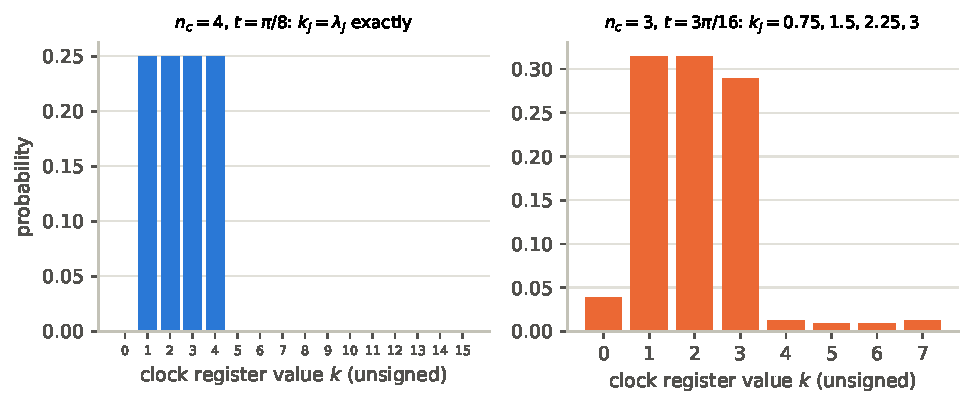
\includegraphics[width=\textwidth]{clock_distribution}\\
      \scriptsize Clock register after QPE for the default system ($b$ has $|\beta_j|^2 = \frac14$ on each eigenvector);
      CUDA-Q state, notebook circuit stopped after QFT$^{-1}$ (re-executed).
    \end{column}
    \begin{column}{0.37\textwidth}
      \small
      \begin{itemize}
        \item General $\phi$: $P(k) = \Big|\frac1M\sum_ce^{2\pi ic(\phi - k/M)}\Big|^2$; the nearest $k$ has $P \ge 4/\pi^2 \approx 0.405$.
        \item Left: $k_j = 1, 2, 3, 4$ exactly, four sharp peaks of $\frac14$.
        \item Right ($n_c = 3$): $k_j = 0.75, 1.5, 2.25, 3$; only $\lambda = 4$ is exact, the rest spread ($P(1) = P(2) = \numpkthree$, $P(3) = \numpkfour$).
      \end{itemize}
    \end{column}
  \end{columns}
\end{frame}

\begin{frame}{Hamiltonian simulation: implementing $e^{iAt}$}
  \begin{columns}[T]
    \begin{column}{0.52\textwidth}
      \small
      \begin{itemize}
        \item For Hermitian $A$, $U = e^{iAt}$ is unitary with eigenvalues $e^{i\lambda_jt}$ on the same eigenvectors $\ket{u_j}$.
        \item \key{Trotter--Suzuki}: $A = \sum_kA_k$ with easy pieces,
          $e^{iAt} \approx \big(\prod_ke^{iA_kt/r}\big)^r$, error $O(t^2/r)$ (first order).
        \item Sparse $A$: decompose into 1-sparse parts; modern methods (qubitization, QSP) reach near-optimal cost.
        \item QPE needs $U^{2^j}$, i.e.\ evolution time up to $2^{n_c-1}t$: total $\sim2^{n_c}t$.
      \end{itemize}
    \end{column}
    \begin{column}{0.44\textwidth}
      \begin{alertblock}{In \texttt{HHL.ipynb}: no Hamiltonian simulation}
        \footnotesize
        \texttt{U\_step = expm(1j * A\_work * t\_evolution)} is the \emph{exact} matrix exponential (SciPy); each
        \texttt{matrix\_power(U, 2**j)} is registered as a custom gate. Fine for a simulator; on hardware this matrix would have to
        be compiled into gates, which is exactly the expensive part.
      \end{alertblock}
    \end{column}
  \end{columns}
\end{frame}

\begin{frame}{Controlled unitary operations}
  \begin{columns}[T]
    \begin{column}{0.5\textwidth}
      \small
      \begin{itemize}
        \item Controlled-$V$: $\ket0\bra0\otimes I + \ket1\bra1\otimes V$.
        \item On an eigenvector, the phase moves onto the control (\key{phase kick-back}):
          $\frac{1}{\sqrt2}(\ket0 + \ket1)\ket u \mapsto \frac{1}{\sqrt2}(\ket0 + e^{i\lambda t2^j}\ket1)\ket u$.
        \item Clock qubit of weight $2^j$ controls $U^{2^j}$: together they apply $U^c$ for clock value $c$.
      \end{itemize}
    \end{column}
    \begin{column}{0.46\textwidth}
      \begin{block}{Notebook convention}
        \footnotesize
        \texttt{clock[0]} is the \key{most significant bit}. The loop applies $U^{2^j}$ controlled by
        \texttt{clock[n\_c - 1 - j]} ($n_c = 4$):\\[1mm]
        \centering
        \begin{tabular}{ccc}
          \toprule $j$ & control & gate\\ \midrule
          0 & \texttt{clock[3]} & $U$\\ 1 & \texttt{clock[2]} & $U^2$\\ 2 & \texttt{clock[1]} & $U^4$\\ 3 & \texttt{clock[0]} & $U^8$\\ \bottomrule
        \end{tabular}\\[1mm]
        \raggedright Custom gates are called as \texttt{kernel.<name>(control, *system)}: the first qubit is the control.
      \end{block}
    \end{column}
  \end{columns}
\end{frame}

\begin{frame}{Eigenvalue estimation for HHL}
  \begin{columns}[T]
    \begin{column}{0.52\textwidth}
      With $U = e^{iAt}$: $\phi_j = \dfrac{\lambda_jt}{2\pi}$, so the clock reads
      \[ k_j = \frac{\lambda_j\,t\,2^{n_c}}{2\pi} = \frac{\lambda_j}{C},\qquad C = \frac{2\pi}{2^{n_c}t}. \]
      \key{Negative eigenvalues} wrap around (two's complement): a register value $k \ge 2^{n_c-1}$ means $k - 2^{n_c}$.
      \small\[ \lt_k = C\cdot\tilde k,\quad \tilde k = \begin{cases}k & k < 2^{n_c-1}\\ k - 2^{n_c} & k \ge 2^{n_c-1}\end{cases} \]
    \end{column}
    \begin{column}{0.44\textwidth}
      \begin{exampleblock}{Default ($n_c = 4$, $t = \pi/8$)}
        $k_j = \lambda_j\cdot\frac{(\pi/8)\cdot16}{2\pi} = \lambda_j$: clock values $1, 2, 3, 4$ (\texttt{0001}, \dots, \texttt{0100}). After QPE:
        \[ \tfrac12\big(\ket{u_1}\ket1 + \ket{u_2}\ket2 + \ket{u_3}\ket3 + \ket{u_4}\ket4\big) \]
      \end{exampleblock}
      \small $n_c = 4$: register 13 (\texttt{1101}) means $\tilde k = -3$; register 8 means $-8$.
    \end{column}
  \end{columns}
\end{frame}

% =====================================================================================
\section{Part 4: The HHL algorithm}
\begin{frame}{The three registers}
  \begin{columns}[T]
    \begin{column}{0.5\textwidth}
      \footnotesize
      \begin{tabular}{p{1.3cm}p{1.1cm}p{3.1cm}}
        \toprule register & qubits & role\\ \midrule
        clock & $n_c = 4$ & phase estimation: holds $\lt_j$ in binary\\
        system & $n_b = 2$ & starts as $\ket b$, ends as $\ket x$\\
        ancilla & 1 & rotated by $C/\lt$; $\ket1$ = success\\ \midrule
        total & 7 & notebook default\\ \bottomrule
      \end{tabular}\\[2mm]
      \small Qubit layout (one register, qubit 0 first): \texttt{clock[0..3]}, \texttt{system[0..1]}, \texttt{ancilla} = qubits 0--3, 4--5, 6.
    \end{column}
    \begin{column}{0.46\textwidth}
      \begin{block}{How many clock qubits?}
        \begin{itemize}
          \item enough levels for all eigenvalues: $\kappa \le 2^{n_c-1} - 1$ (notebook's ``auto'' condition)
          \item precision $\varepsilon$: $n_c \approx \log_2(\kappa/\varepsilon)$ + a few
          \item default $\kappa = 4 \le 7$: $n_c = 4$ suffices, every $k_j$ exact
        \end{itemize}
      \end{block}
      \small Total qubits $n_b + n_c + 1$.
    \end{column}
  \end{columns}
\end{frame}

\begin{frame}{The state, step by step}
  \footnotesize
  \begin{tabular}{p{3.1cm}p{9.9cm}}
    \toprule step & state (eigenbasis of $A$; clock value $k_j = \lambda_j/C$ assumed exact)\\ \midrule
    0.\ initial & $\ket0_c\,\ket b\,\ket0_a = \sum_j\beta_j\ket0_c\ket{u_j}\ket0_a$\\[1mm]
    1.\ $H^{\otimes n_c}$ + controlled $U^{2^j}$ & $\sum_j\beta_j\frac{1}{\sqrt M}\sum_ce^{i\lambda_jtc}\ket c\ket{u_j}\ket0_a$\\[1mm]
    2.\ QFT$^{-1}$ (end of QPE) & $\sum_j\beta_j\ket{k_j}\ket{u_j}\ket0_a$\\[1mm]
    3.\ controlled $R_Y(\theta_k)$ & $\sum_j\beta_j\ket{k_j}\ket{u_j}\Big(\sqrt{1 - \frac{C^2}{\lambda_j^2}}\ket0 + \frac{C}{\lambda_j}\ket1\Big)$\\[1mm]
    4.\ QPE$^{-1}$ (uncompute) & $\sum_j\beta_j\ket0_c\ket{u_j}\Big(\sqrt{1 - \frac{C^2}{\lambda_j^2}}\ket0 + \frac{C}{\lambda_j}\ket1\Big)$\\[1mm]
    5.\ measure ancilla $= 1$ & $\dfrac{C\sum_j\frac{\beta_j}{\lambda_j}\ket{u_j}}{\sqrt{P_{\text{success}}}} = \ket x$,\qquad $P_{\text{success}} = C^2\sum_j\frac{|\beta_j|^2}{\lambda_j^2} = C^2\|A^{-1}\ket b\|^2$\\ \bottomrule
  \end{tabular}\\[2mm]
  The un-normalised branch ``clock $= 0$, ancilla $= 1$'' is $C\,A^{-1}\ket b$ --- the notebook reads exactly these amplitudes.
\end{frame}

\begin{frame}{Eigenvalue inversion}
  \begin{columns}[T]
    \begin{column}{0.52\textwidth}
      \begin{block}{The rotation}
        \[ R_Y(\theta)\ket0 = \cos\tfrac\theta2\ket0 + \sin\tfrac\theta2\ket1 \]
        Choose $\theta_k = 2\arcsin\dfrac{C}{\lt_k}$ $\Rightarrow$ amplitude $\dfrac{C}{\lt_k}$ on $\ket1$.
      \end{block}
      \small
      \begin{itemize}
        \item $C$ must satisfy $|C/\lt| \le 1$ for all eigenvalues: $C \le |\lambda|_{\min}$.
        \item Larger $C$ $\Rightarrow$ higher success probability; the best choice is $C = |\lambda|_{\min}$.
        \item Negative $\lt$ gives a negative angle: the sign of $1/\lambda$ is kept.
      \end{itemize}
    \end{column}
    \begin{column}{0.44\textwidth}
      \begin{block}{The approximation constant $C$}
        In the notebook $C = 2\pi/(2^{n_c}t)$ = the eigenvalue of clock value 1, i.e.\ the smallest representable $|\lt|$.
        Default: $C = 1 = \lambda_{\min}$.
      \end{block}
      \begin{exampleblock}{Default angles}
        \footnotesize $\lt = 1, 2, 3, 4$: $\sin\frac\theta2 = 1, \frac12, \frac13, \frac14$;
        $\theta = \pi,\ \frac\pi3,\ 0.6797,\ 0.5054$ rad.
      \end{exampleblock}
    \end{column}
  \end{columns}
\end{frame}

\begin{frame}{Controlled rotation: the notebook's lookup table}
  \begin{columns}[c]
    \begin{column}{0.56\textwidth}
      \centering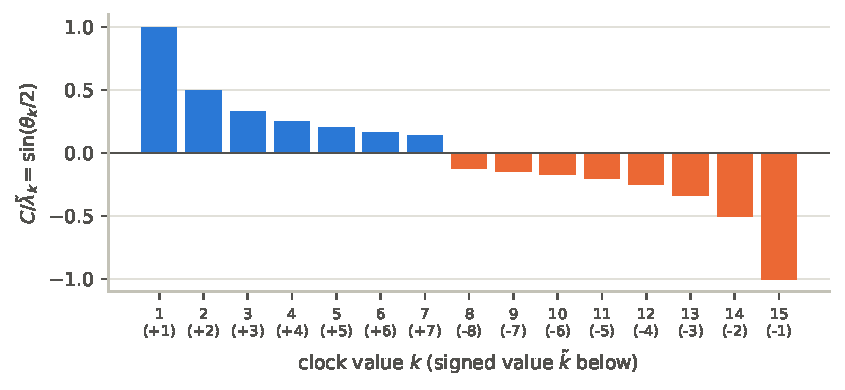
\includegraphics[width=\textwidth]{inversion_table}\\
      \scriptsize $n_c = 4$, $t = \pi/8$, $C = 1$: amplitude $C/\lt_k = 1/\tilde k$ for all 15 non-zero clock values.
    \end{column}
    \begin{column}{0.41\textwidth}
      \small
      \begin{itemize}
        \item For every $k = 1, \dots, 2^{n_c} - 1$: flip the clock qubits that are 0 in $k$ (\texttt{x} ``polarity'' gates), apply
          $R_Y(\theta_k)$ controlled on \emph{all} clock qubits (\texttt{ccccry}), flip back.
        \item $k = 0$ is skipped (no eigenvalue 0).
        \item Default: 15 \texttt{ccccry} + 56 \texttt{x} gates.
        \item Cost grows like $2^{n_c}$; scalable versions compute $1/\lt$ arithmetically.
      \end{itemize}
    \end{column}
  \end{columns}
\end{frame}

\begin{frame}{The ancilla qubit}
  \begin{columns}[T]
    \begin{column}{0.5\textwidth}
      \begin{itemize}
        \item One extra qubit, initially $\ket0$.
        \item After the rotation, for eigenvalue $\lambda_j$:
          \[ \sqrt{1 - \tfrac{C^2}{\lambda_j^2}}\ket0 + \tfrac{C}{\lambda_j}\ket1 \]
        \item $\ket1$ \emph{flags} the branch in which the system carries $A^{-1}$.
        \item Small eigenvalues get large $\ket1$-amplitudes: this is how $1/\lambda$ is ``divided'' with a unitary.
      \end{itemize}
    \end{column}
    \begin{column}{0.46\textwidth}
      \begin{alertblock}{Why not apply $A^{-1}$ directly?}
        $A^{-1}$ is not unitary. HHL embeds it as one block of a larger unitary; the price is a \key{probabilistic} outcome:
        the $\ket1$ branch must be selected by measurement.
      \end{alertblock}
      \small Probability of ancilla $= 1$ for a single eigenvector $\ket{u_j}$: $C^2/\lambda_j^2$ (e.g.\ $\lambda = 4$, $C = 1$: $1/16$).
    \end{column}
  \end{columns}
\end{frame}

\begin{frame}{Uncomputation}
  \begin{columns}[T]
    \begin{column}{0.5\textwidth}
      After step 3 the clock is \key{entangled} with the system:
      \[ \sum_j\beta_j\ket{k_j}\ket{u_j}\big(\cdots\ket0 + \tfrac{C}{\lambda_j}\ket1\big). \]
      If we post-selected now, the system would be in a \hl{mixture}, not in $\ket x$: the different $\ket{k_j}$ are orthogonal,
      so the terms cannot interfere.
    \end{column}
    \begin{column}{0.46\textwidth}
      \begin{block}{Inverse QPE}
        Apply QFT, then controlled $U^{-2^j}$, then $H^{\otimes n_c}$: every $\ket{k_j}\ket{u_j}$ returns to $\ket0\ket{u_j}$.
        The clock factors out and the system holds the coherent superposition $\sum_j\beta_j\frac{C}{\lambda_j}\ket{u_j}$.
      \end{block}
      \small Notebook: \texttt{h} + \texttt{cr1}$(+\pi/2^{k-j})$, swaps, \texttt{matrix\_power(U.conj().T, 2**j)}, \texttt{h}.
      If phases are inexact the clock does not return perfectly to $\ket0$; the notebook post-selects clock $= 0$ \emph{and} ancilla $= 1$.
    \end{column}
  \end{columns}
\end{frame}

\begin{frame}{HHL circuit architecture}
  \centering
  \resizebox{0.97\linewidth}{!}{%
  \begin{quantikz}[row sep=0.45cm, column sep=0.35cm]
    \lstick{clock $\ket0^{\otimes n_c}$} & \qwbundle{n_c} & \gate{H^{\otimes n_c}} & \ctrl{1} & \gate{\mathrm{QFT}^{-1}} & \ctrl{2} & \gate{\mathrm{QFT}} & \ctrl{1} & \gate{H^{\otimes n_c}} & \meter{} & \rstick{$=0$}\\
    \lstick{system $\ket b$} & \qwbundle{n_b} & \qw & \gate{U^c} & \qw & \qw & \qw & \gate{U^{-c}} & \qw & \meter{} & \rstick{$\sim|x_i|^2$}\\
    \lstick{ancilla $\ket0$} & \qw & \qw & \qw & \qw & \gate{R_Y(\theta_k)} & \qw & \qw & \qw & \meter{} & \rstick{$=1$}
  \end{quantikz}}\\[3mm]
  \begin{columns}[T]
    \begin{column}{0.32\textwidth}\centering\small \key{QPE}: $H$, controlled $U^{2^j}$, QFT$^{-1}$\end{column}
    \begin{column}{0.32\textwidth}\centering\small \key{Inversion}: $2^{n_c} - 1$ multi-controlled $R_Y$\end{column}
    \begin{column}{0.32\textwidth}\centering\small \key{Uncompute}: QFT, controlled $U^{-2^j}$, $H$\end{column}
  \end{columns}
  \vspace{2mm}
  \small ``controlled $U^c$'' = the $n_c$ gates $U^{2^j}$, each controlled by one clock qubit. The notebook measures all qubits (\texttt{mz(reg)}).
\end{frame}

\begin{frame}{Measurement and post-selection}
  \begin{columns}[T]
    \begin{column}{0.52\textwidth}
      \begin{block}{Success probability}
        \[ P_{\text{success}} = \sum_j|\beta_j|^2\frac{C^2}{\lambda_j^2} = C^2\,\|A^{-1}\ket b\|^2 \]
        Expected repetitions: $1/P_{\text{success}}$.
      \end{block}
      \small
      \begin{itemize}
        \item $C \le |\lambda|_{\min}$ and $|\lambda| \le |\lambda|_{\max}$ give $P_{\text{success}} \ge 1/\kappa^2$.
        \item \key{Amplitude amplification} reduces $O(\kappa^2)$ repetitions to $O(\kappa)$.
      \end{itemize}
    \end{column}
    \begin{column}{0.44\textwidth}
      \begin{exampleblock}{Default system (exact)}
        $|\beta_j|^2 = \frac14$, $C = 1$:
        \[ P = \tfrac14\big(1 + \tfrac14 + \tfrac19 + \tfrac1{16}\big) = \tfrac{205}{576} \]
        $= 0.355903$.
        $20\,000$ shots $\Rightarrow$ about $7118$ accepted. Recorded: $7086$ ($0.3543$).
      \end{exampleblock}
      \small Notebook filter: \texttt{bits[:n\_c] == "0000"} and \texttt{bits[-1] == "1"}.
    \end{column}
  \end{columns}
\end{frame}

\begin{frame}{Extracting information about the solution}
  \begin{columns}[T]
    \begin{column}{0.5\textwidth}
      \small
      \begin{itemize}
        \item \key{Sampling}: accepted shots give $i$ with probability $|x_i|^2/\|x\|^2$ --- magnitudes only, error $\sim1/\sqrt{\text{accepted}}$.
        \item \key{Signs / phases}: need other bases or interference with a reference state.
        \item \key{Norm}: $\|A^{-1}\ket b\| = \sqrt{P_{\text{success}}}/C$, so $P_{\text{success}}$ estimates it.
        \item \key{Expectation values} $\braket{x|M|x}$ and overlaps: the intended use.
        \item Full vector: $O(d/\varepsilon^2)$ shots --- no advantage over classical solvers.
      \end{itemize}
    \end{column}
    \begin{column}{0.46\textwidth}
      \begin{block}{Notebook: norm recovery (simulator only)}
        The state vector is read with \texttt{cudaq.get\_state}; the branch clock $= 0$, ancilla $= 1$ has amplitudes $C\,A^{-1}b/\|b\|$, so
        \[ x = \frac{\|b\|}{C}\times\text{amplitudes}. \]
        This uses full amplitude access, which hardware does not provide.
      \end{block}
    \end{column}
  \end{columns}
\end{frame}

\begin{frame}[fragile]{HHL in pseudocode}
  \begin{columns}[T]
    \begin{column}{0.56\textwidth}
\begin{lstlisting}[language={},basicstyle=\ttfamily\tiny]
input: Hermitian A (d x d), b, clock qubits n_c, time t
C <- 2*pi / (2^n_c * t)
prepare |0>_clock |b>_system |0>_ancilla
# 1) phase estimation
H on every clock qubit
for j = 0 .. n_c-1: controlled-U^(2^j), U = exp(iAt)
inverse QFT on the clock
# 2) eigenvalue inversion
for k = 1 .. 2^n_c - 1:
    lam_k <- C * signed(k)
    if clock == k: RY(2 arcsin(C/lam_k)) on ancilla
# 3) uncompute: QFT, controlled-U^(-2^j), H
# 4) measure; keep shots with clock = 0, ancilla = 1
return system register  (state |x>)
\end{lstlisting}
    \end{column}
    \begin{column}{0.40\textwidth}
      \begin{block}{Expected measurement outcomes}
        \small
        \begin{itemize}
          \item ancilla $= 1$ with probability $P_{\text{success}}$
          \item clock $= 0$ whenever ancilla $= 1$ (exact phases)
          \item system: $i$ with probability $|x_i|^2/\|x\|^2$ among accepted shots
        \end{itemize}
      \end{block}
    \end{column}
  \end{columns}
\end{frame}

% =====================================================================================
\section{Part 5: Worked examples}
\begin{frame}{Worked example 1: a $2\times2$ system --- set-up}
  \begin{columns}[T]
    \begin{column}{0.5\textwidth}
      \small $A = \begin{psmallmatrix}1&-1/3\\-1/3&1\end{psmallmatrix}$, $b = (1, 0)$ (notebook, Section 4 table).
      \begin{enumerate}
        \item $\lambda_1 = \frac23$, $\ket{u_1} = \frac{1}{\sqrt2}(1, 1)$; $\lambda_2 = \frac43$, $\ket{u_2} = \frac{1}{\sqrt2}(1, -1)$; $\kappa = 2$.
        \item $\beta_1 = \beta_2 = \frac{1}{\sqrt2}$.
        \item $n_c = 4$, $k_{\max} = 7 \ge \kappa$: $t = \dfrac{2\pi}{16\cdot\frac23} = \dfrac{3\pi}{16}$, $C = \frac23$.
        \item Clock values $k_j = \lambda_j/C = 1, 2$ (exact).
      \end{enumerate}
    \end{column}
    \begin{column}{0.46\textwidth}
      \begin{block}{After QPE}
        \[ \tfrac{1}{\sqrt2}\ket{0001}\ket{u_1}\ket0 + \tfrac{1}{\sqrt2}\ket{0010}\ket{u_2}\ket0 \]
      \end{block}
      \begin{block}{Rotation amplitudes}
        $C/\lambda_1 = 1$ ($\theta = \pi$),\ \ $C/\lambda_2 = \frac12$ ($\theta = \frac\pi3$).
      \end{block}
      \small Registers: 4 clock + 1 system + 1 ancilla = 6 qubits.
    \end{column}
  \end{columns}
\end{frame}

\begin{frame}{Worked example 1: inversion, post-selection, read-out}
  \begin{columns}[T]
    \begin{column}{0.52\textwidth}
      \small After inversion and uncomputation, the ancilla-$\ket1$ branch is
      \begin{align*}
        &\tfrac{1}{\sqrt2}\cdot1\cdot\ket{u_1} + \tfrac{1}{\sqrt2}\cdot\tfrac12\ket{u_2}\\
        &= \tfrac12(1, 1) + \tfrac14(1, -1) = \left(\tfrac34, \tfrac14\right).
      \end{align*}
      \begin{itemize}
        \item $P_{\text{success}} = \frac9{16} + \frac1{16} = \frac58 = 0.625$
        \item $\ket x = \frac{1}{\sqrt{10}}(3, 1)$; shots: $P(0) = 0.9$, $P(1) = 0.1$
        \item norm recovery: $x = \frac{\|b\|}{C}\left(\tfrac34, \tfrac14\right) = \tfrac32\left(\tfrac34, \tfrac14\right)$\\ $= (1.125,\ 0.375)$ \checkmark
      \end{itemize}
    \end{column}
    \begin{column}{0.44\textwidth}
      \begin{exampleblock}{Re-executed with CUDA-Q}
        Notebook circuit, $n_c = 4$, $t = 3\pi/16$:\\
        $P_{\text{success}} = \numptwobytwo$, fidelity $\numfidtwobytwo$, $x = (1.125, 0.375)$ to $10^{-12}$.
      \end{exampleblock}
      \small Check: $C^2\|x\|^2 = \frac49\cdot\frac{90}{64} = 0.625$.
    \end{column}
  \end{columns}
\end{frame}

\begin{frame}{Worked example 2: the notebook's $4\times4$ system --- set-up}
  \begin{columns}[T]
    \begin{column}{0.5\textwidth}
      \small $A = H\,\mathrm{diag}(1, 2, 3, 4)\,H$, $b = (1, 0, 0, 0)$.
      \begin{enumerate}
        \item Eigenvectors = columns of $H$: $\ket{u_j} = H\ket j$, $\lambda_j = 1, 2, 3, 4$; $\kappa = 4$.
        \item $\beta_j = \braket{u_j|b} = H_{0j} = \frac12$ for all $j$.
        \item $n_c = 4$, $k_{\max} = 7$: $t = \pi/8$, $C = 1$, $k_j = \lambda_j$.
        \item 7 qubits: clock 4, system 2, ancilla 1.
      \end{enumerate}
    \end{column}
    \begin{column}{0.46\textwidth}
      \begin{block}{Recorded notebook output (Section 4)}
        \footnotesize
        Eigenvalues $[1, 2, 3, 4]$, $\kappa = 4.0000$\\
        $t = 0.392699$ ($=\pi/8$), $C = 1.000000$\\
        clock values $+1.000, +2.000, +3.000, +4.000$ (exact)\\
        $n_b + n_c + 1 = 2 + 4 + 1 = 7$ qubits
      \end{block}
    \end{column}
  \end{columns}
\end{frame}

\begin{frame}{Worked example 2: the solution by hand}
  \begin{columns}[T]
    \begin{column}{0.58\textwidth}
      \small Post-selected branch: $\sum_j\frac12\cdot\frac1{\lambda_j}\ket{u_j} = H\cdot\frac12\left(1, \tfrac12, \tfrac13, \tfrac14\right)$:
      \begin{align*}
        x &= \tfrac14\big(1 + \tfrac12 + \tfrac13 + \tfrac14,\ 1 - \tfrac12 + \tfrac13 - \tfrac14,\\
          &\qquad\ \ 1 + \tfrac12 - \tfrac13 - \tfrac14,\ 1 - \tfrac12 - \tfrac13 + \tfrac14\big)\\
          &= \tfrac{1}{48}(25, 7, 11, 5)\\
          &= (0.520833,\ 0.145833,\ 0.229167,\ 0.104167)
      \end{align*}
      \begin{itemize}
        \item $C = \|b\| = 1$, so the amplitudes \emph{are} $x$.
        \item $P = \|x\|^2 = \frac{820}{2304} = \frac{205}{576} = 0.355903$.
        \item $|x_i|^2/\|x\|^2 = \frac{(625, 49, 121, 25)}{820}$\\ $= (0.7622, 0.0598, 0.1476, 0.0305)$.
      \end{itemize}
    \end{column}
    \begin{column}{0.38\textwidth}
      \begin{exampleblock}{Recorded = re-executed}
        \footnotesize
        \begin{tabular}{lcc}
          \toprule & NumPy & HHL state\\ \midrule
          $x_0$ & 0.520833 & 0.520833\\ $x_1$ & 0.145833 & 0.145833\\ $x_2$ & 0.229167 & 0.229167\\ $x_3$ & 0.104167 & 0.104167\\ \bottomrule
        \end{tabular}\\[1mm]
        fidelity $1.0000000000$
      \end{exampleblock}
    \end{column}
  \end{columns}
\end{frame}

% =====================================================================================
\section{Part 6: Complexity}
\begin{frame}{Complexity analysis}
  \begin{columns}[T]
    \begin{column}{0.54\textwidth}
      \begin{block}{HHL (2009)}
        \[ \tilde O\!\left(\log(d)\,\frac{s^2\kappa^2}{\varepsilon}\right) \]
        $\log d$: amplitude encoding + sparse Hamiltonian simulation.\\
        $\kappa$: one factor from QPE precision, one from $P_{\text{success}}$ (with amplitude amplification).\\
        $1/\varepsilon$: phase-estimation precision.
      \end{block}
    \end{column}
    \begin{column}{0.42\textwidth}
      \small
      \begin{tabular}{ll}
        \toprule & cost\\ \midrule
        dense LU & $O(d^3)$\\
        CG (PD) & $O(d\,s\sqrt\kappa\log\frac1\varepsilon)$\\
        HHL & $\tilde O(\log(d)s^2\kappa^2/\varepsilon)$\\ \bottomrule
      \end{tabular}\\[2mm]
      Exponential in $d$ \emph{only if} $s$, $\kappa$ and $1/\varepsilon$ are $\mathrm{polylog}(d)$, $\ket b$ is cheap, and only a property of $\ket x$
      is needed.
    \end{column}
  \end{columns}
\end{frame}

\begin{frame}{Sparsity and condition-number dependence}
  \begin{columns}[c]
    \begin{column}{0.5\textwidth}
      \centering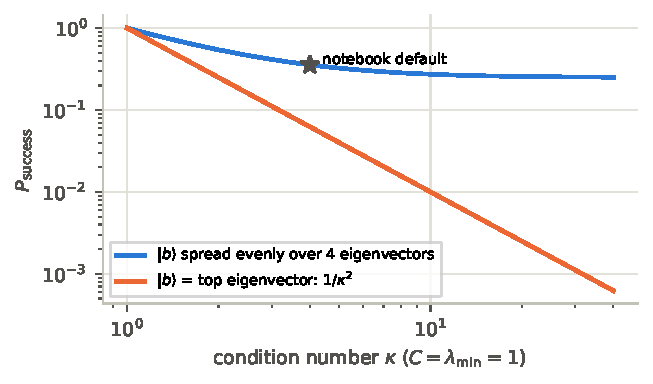
\includegraphics[width=\textwidth]{kappa_success}\\
      \scriptsize Illustrative (NumPy, formula $P = \sum_j|\beta_j|^2C^2/\lambda_j^2$, $C = \lambda_{\min} = 1$).
    \end{column}
    \begin{column}{0.46\textwidth}
      \small
      \begin{itemize}
        \item $P_{\text{success}}$ depends on where $b$ lives: worst case $1/\kappa^2$ (all weight on $\lambda_{\max}$).
        \item Clock qubits: $n_c \gtrsim \log_2\kappa$ just to resolve $\lambda_{\min}$ next to $\lambda_{\max}$.
        \item Sparsity $s$ enters through Hamiltonian simulation (original analysis $s^2$; modern methods $\approx s$).
        \item Dense $A$ ($s = d$) destroys the $\log d$ scaling.
        \item \key{Preconditioning} can reduce $\kappa$ (an active research topic).
      \end{itemize}
    \end{column}
  \end{columns}
\end{frame}

\begin{frame}{Theoretical speed-up versus practical advantage}
  \begin{columns}[T]
    \begin{column}{0.5\textwidth}
      \begin{alertblock}{The fine print (Aaronson, Nature Physics 2015)}
        \small
        \begin{enumerate}
          \item \key{Input}: loading a generic $b$ costs $O(d)$.
          \item \key{Matrix}: $e^{iAt}$ must be efficient --- sparse or structured $A$.
          \item \key{Conditioning}: $\kappa$ must be small.
          \item \key{Output}: you get $\ket x$, not $x$.
        \end{enumerate}
      \end{alertblock}
    \end{column}
    \begin{column}{0.46\textwidth}
      \small
      \begin{itemize}
        \item \key{Dequantisation} (Tang 2018 and later): for low-rank problems with sampling access, classical algorithms match the quantum scaling up to polynomial factors.
        \item HHL is \key{BQP-complete}: an efficient classical simulation of all HHL instances would simulate all quantum computers.
        \item No practical advantage for linear systems has been demonstrated; fault tolerance is needed.
      \end{itemize}
    \end{column}
  \end{columns}
\end{frame}

% =====================================================================================
\section{Part 7: CUDA-Q implementation}
\begin{frame}{\texttt{HHL.ipynb}: structure and parameters}
  \begin{columns}[T]
    \begin{column}{0.46\textwidth}
      \scriptsize
      \begin{tabular}{rl}
        \toprule \S & content\\ \midrule
        1 & problem and mathematics\\ 2 & imports, version checks\\ 3 & \textbf{input parameters (only cell to edit)}\\
        4 & build, validate, embed/pad; $t$, $C$, qubits\\ 5 & benchmark utilities, backend\\ 6 & expected output (before running)\\
        7 & circuit builder, drawing, statistics\\ 8 & execution with memory monitor\\ 9 & results and plots\\ 10 & benchmark report\\ \bottomrule
      \end{tabular}
    \end{column}
    \begin{column}{0.5\textwidth}
      \scriptsize
      \begin{tabular}{ll}
        \toprule parameter & default\\ \midrule
        \texttt{MATRIX\_A}, \texttt{VECTOR\_B} & \texttt{"example"}\\
        \texttt{NUM\_CLOCK\_QUBITS} & 4\\
        \texttt{EVOLUTION\_TIME} & \texttt{"auto"}\\
        \texttt{BACKEND} & \texttt{"auto"}\\
        \texttt{SIMULATION\_METHOD} & \texttt{"statevector"}\\
        \texttt{SHOTS}, \texttt{SEED} & 20000, 42\\ \bottomrule
      \end{tabular}\\[2mm]
      Allowed methods: \texttt{"statevector"}, \texttt{"density\_matrix"}.
      Validation: square $A$, matching $b$, $b \ne 0$, $|\det A| \ge 10^{-12}$ and $\mathrm{cond}(A) \le 10^{12}$; $n_c \ge 2$.
    \end{column}
  \end{columns}
\end{frame}

\begin{frame}[fragile]{Section 4: making the system HHL-ready}
\begin{lstlisting}[basicstyle=\ttfamily\tiny]
H4 = 0.5 * np.array([[1, 1, 1, 1], [1, -1, 1, -1], [1, 1, -1, -1], [1, -1, -1, 1]])
A_input = H4 @ np.diag([1.0, 2.0, 3.0, 4.0]) @ H4            # eigenvalues exactly 1, 2, 3, 4
x_classical = np.linalg.solve(A_input, b_input)               # reference solution
if not hermitian:                                             # [[0, A], [A^dag, 0]] [y; x] = [b; 0]
    A_work = np.block([[np.zeros((d0, d0)), A_work], [A_work.conj().T, np.zeros((d0, d0))]])
...
k_max = 2 ** (n_c - 1) - 1                                    # largest positive clock value (signed)
if kappa <= k_max:
    t_evolution = 2 * np.pi / (2 ** n_c * lam_abs_min)        # smallest |lambda| -> clock value 1
else:
    t_evolution = 2 * np.pi * k_max / (2 ** n_c * lam_abs_max)
C_constant = 2 * np.pi / (2 ** n_c * t_evolution)             # smallest representable |eigenvalue|
total_qubits = n_c + n_b + 1
\end{lstlisting}
  \small Excerpt (comments shortened). Everything after this cell reads $n_c$, $n_b$, $t$ and $C$ from here.
\end{frame}

\begin{frame}[fragile]{Section 7a: the circuit --- phase estimation}
  \begin{columns}[T]
    \begin{column}{0.62\textwidth}
\begin{lstlisting}[basicstyle=\ttfamily\tiny]
U_step = expm(1j * A_work * t_evolution)     # exact exp(iAt)
kernel = cudaq.make_kernel()
reg = kernel.qalloc(bit_reverse_order(initial, n_tot))
clock = [reg[i] for i in range(nc)]
system = [reg[nc + i] for i in range(n_b)]
ancilla = reg[n_tot - 1]
for q in clock:
    kernel.h(q)
for j in range(nc):
    name = f"hhl_{gate_uid}_{nc}_u{j}"
    cudaq.register_operation(name, np.linalg.matrix_power(U, 2 ** j))
    getattr(kernel, name)(clock[nc - 1 - j], *system)
for j in range(nc // 2):                     # inverse QFT
    kernel.swap(clock[j], clock[nc - 1 - j])
for jj in range(nc):
    j = nc - 1 - jj
    for kk in range(nc - 1 - j):
        k = nc - 1 - kk
        kernel.cr1(-np.pi / 2 ** (k - j), clock[k], clock[j])
    kernel.h(clock[j])
\end{lstlisting}
    \end{column}
    \begin{column}{0.35\textwidth}
      \small
      \begin{itemize}
        \item \key{Kernel builder} (\texttt{make\_kernel}): needed because each $U^{2^j}$ is a new custom gate.
        \item \texttt{initial} $= \ket{0}_c\otimes\ket b\otimes\ket0_a$, bit-reversed because CUDA-Q indexes qubit 0 as the least significant bit.
        \item The first argument of the custom gate is the control.
      \end{itemize}
    \end{column}
  \end{columns}
\end{frame}

\begin{frame}[fragile]{Section 7a: inversion, uncomputation, read-out}
  \begin{columns}[T]
    \begin{column}{0.62\textwidth}
\begin{lstlisting}[basicstyle=\ttfamily\tiny]
for k_val in range(1, 2 ** nc):
    signed = k_val - 2 ** nc if k_val >= 2 ** (nc - 1) else k_val
    lam_k = 2 * np.pi * signed / (2 ** nc * t_used)
    theta = 2 * np.arcsin(np.clip(c_used / lam_k, -1.0, 1.0))
    zero_bits = [i for i in range(nc) if not (k_val >> (nc - 1 - i)) & 1]
    for i in zero_bits: kernel.x(clock[i])
    kernel.cry(theta, clock, ancilla)        # multi-controlled
    for i in zero_bits: kernel.x(clock[i])
# uncompute: QFT, swaps, U^-(2^j), H   (mirror image)
...
def postselected_amplitudes(state_vector):
    tensor = np.asarray(state_vector).reshape([2] * total_qubits) \
               .transpose(list(range(total_qubits))[::-1])
    return tensor[(0,) * n_c + (slice(None),) * n_b + (1,)].reshape(-1)
x_quantum_full = amplitudes * b_norm / C_constant   # norm recovery
\end{lstlisting}
    \end{column}
    \begin{column}{0.35\textwidth}
      \small
      \begin{itemize}
        \item \texttt{signed}: two's complement for negative eigenvalues.
        \item \texttt{np.clip} guards $|C/\lt| \le 1$.
        \item \texttt{kernel.cry(theta, clock, ancilla)} with a list of controls becomes \texttt{ccccry} for $n_c = 4$.
        \item Read-out: the branch clock $= 0$, ancilla $= 1$, then $x = \|b\|/C\cdot$ amplitudes.
      \end{itemize}
    \end{column}
  \end{columns}
\end{frame}

\begin{frame}{Circuit statistics (\texttt{cudaq.estimate\_resources})}
  \begin{columns}[c]
    \begin{column}{0.48\textwidth}
      \centering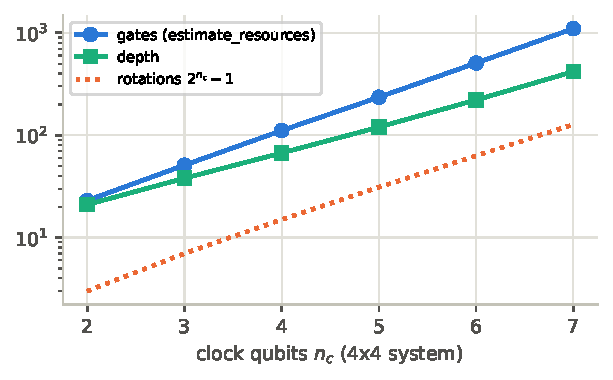
\includegraphics[width=\textwidth]{circuit_size}
    \end{column}
    \begin{column}{0.48\textwidth}
      \small
      \begin{center}
      \begin{tabular}{ccccc}
        \toprule $n_c$ & qubits & gates & rotations & depth\\ \midrule
        \numgatesrows \bottomrule
      \end{tabular}
      \end{center}
      \scriptsize 4$\times$4 system, ``auto'' time, measurements and the amplitude loading of $\ket b$ not counted (as in the notebook).
      Recorded default ($n_c = 4$): 111 gates = \texttt{h} 16, custom 8, \texttt{swap} 4, \texttt{cr1} 12, \texttt{x} 56, \texttt{ccccry} 15; 39 multi-qubit; depth 67.
      The notebook's pre-run estimate ``$\sim$107 gates'' is a formula, not a count.
    \end{column}
  \end{columns}
\end{frame}

\begin{frame}{Recorded results of the default run}
  \begin{columns}[c]
    \begin{column}{0.56\textwidth}
      \centering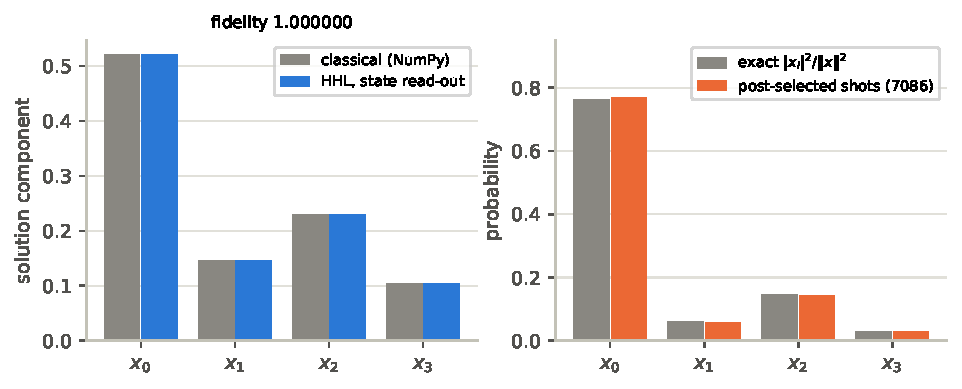
\includegraphics[width=\textwidth]{default_solution}\\
      \scriptsize Re-executed with the notebook's circuit and seed 42; identical to the recorded output.
    \end{column}
    \begin{column}{0.41\textwidth}
      \small
      \begin{itemize}
        \item State read-out: $x$ equals NumPy's solution; fidelity $1.0000000000$; relative error $1.655\times10^{-15}$ (recorded).
        \item Shots: $7086$ of $20\,000$ accepted ($P = 0.3543$ vs.\ $0.3559$).
        \item Sampled $|x_i|^2$:\\ $(\numsampledrow)$;\\ max.\ error $\numshotmax$ vs.\ statistical scale $\pm\numstaterr$.
      \end{itemize}
    \end{column}
  \end{columns}
\end{frame}

\begin{frame}{Recorded, re-executed and variant runs}
  \footnotesize
  \begin{center}
  \resizebox{\linewidth}{!}{%
  \begin{tabular}{p{3.6cm}p{3.2cm}cccc}
    \toprule run & settings & $C$ & $P_{\text{success}}$ (state) & fidelity & accepted shots\\ \midrule
    \textbf{recorded} (notebook output) & default, $n_c = 4$, $t = \pi/8$ & 1 & 0.355903 & 1.0000000000 & 7086 / 20000\\
    \textbf{re-executed} (CUDA-Q 0.16, \texttt{qpp-cpu}, seed 42) & same & 1 & \numpstate & \numfiddef & \numacc{} / 20000\\
    variant, re-executed & default $A$, $n_c = 3$, $t = 3\pi/16$ & $\numcthree$ & \numpthree & \numfidthree & ---\\
    variant, re-executed & default $A$, $n_c = 2$, $t = \pi/8$ & 4 & \numptwo & \numfidtwo & ---\\
    variant, re-executed & $2\times2$ example, $n_c = 4$ & $\frac23$ & \numptwobytwo & \numfidtwobytwo & ---\\ \bottomrule
  \end{tabular}}
  \end{center}
  \begin{itemize}
    \item Relative error of the re-executed default: $\numrelerr$ (recorded $1.655\times10^{-15}$): floating-point level.
    \item Variants change only Section 3 parameters; the circuit code is the notebook's.
    \item Recorded timings (CPU, \texttt{qpp-cpu}): construction 0.0056 s, compilation 0.0524 s, state run 0.0018 s, sampling 0.0758 s.
  \end{itemize}
\end{frame}

\begin{frame}{Precision: what too few clock qubits do}
  \begin{columns}[c]
    \begin{column}{0.55\textwidth}
      \centering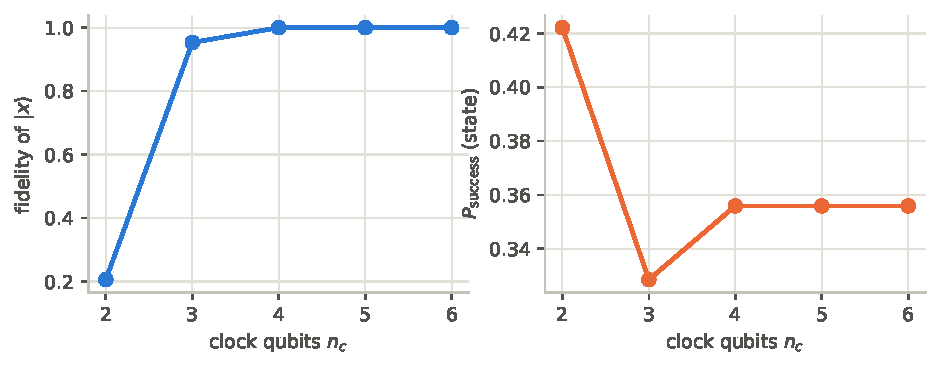
\includegraphics[width=\textwidth]{precision}\\
      \scriptsize Default system, ``auto'' time, CUDA-Q state read-out (re-executed).
    \end{column}
    \begin{column}{0.42\textwidth}
      \small
      \begin{itemize}
        \item $n_c = 3$: $\kappa = 4 > k_{\max} = 3$, so $\lambda_{\max}\to3$, $t = 3\pi/16$, $C = \frac43$; clock values $0.75, 1.5, 2.25, 3$ are rounded:
          fidelity $\numfidthree$.
        \item $n_c \ge 4$: every $k_j$ is an integer, fidelity 1.
      \end{itemize}
      \begin{alertblock}{Finding in the notebook}
        \scriptsize For $n_c = 3$ the notebook prints an ``ideal'' $P_{\text{success}} = \numidealthree$ from $\sum_j|\beta_j|^2C^2/\lambda_j^2$.
        With $C = \frac43 > \lambda_{\min}$ this formula is not a probability ($C/\lambda_1 > 1$); the circuit gives $\numpthree$.
      \end{alertblock}
    \end{column}
  \end{columns}
\end{frame}

\begin{frame}{Shot noise of the read-out}
  \begin{columns}[c]
    \begin{column}{0.5\textwidth}
      \centering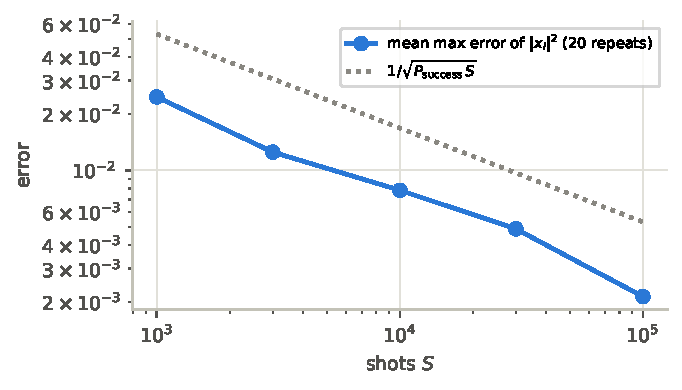
\includegraphics[width=\textwidth]{shot_noise}\\
      \scriptsize 20 repeated samplings per shot count, notebook circuit (re-executed).
    \end{column}
    \begin{column}{0.46\textwidth}
      \small
      \begin{itemize}
        \item Only accepted shots ($\approx35.6\,\%$) carry information about $\ket x$.
        \item Error of each estimated $|x_i|^2$ scales as $1/\sqrt{P_{\text{success}}\cdot S}$.
        \item $20\,000$ shots $\to$ $\approx7100$ accepted $\to$ $\pm0.012$.
        \item Halving the error costs $4\times$ the shots --- the read-out cost behind ``$d/\varepsilon^2$''.
      \end{itemize}
    \end{column}
  \end{columns}
\end{frame}

\begin{frame}{CPU and GPU simulation}
  \begin{columns}[T]
    \begin{column}{0.58\textwidth}
      \scriptsize
      \resizebox{\linewidth}{!}{%
      \begin{tabular}{lll}
        \toprule choice & CUDA-Q target & note\\ \midrule
        \texttt{cpu} + \texttt{statevector} & \texttt{qpp-cpu} & fp64\\
        \texttt{cpu} + \texttt{density\_matrix} & \texttt{density-matrix-cpu} & $4^N$ memory\\
        \texttt{gpu} + \texttt{statevector} & \texttt{nvidia} & fp32/fp64\\
        \texttt{multi-gpu} + \texttt{statevector} & \texttt{nvidia} (\texttt{mgpu}) & needs MPI\\
        \texttt{hardware} & provider & \hl{refused by HHL.ipynb}\\ \bottomrule
      \end{tabular}}\\[2mm]
      \small \texttt{BACKEND = "auto"} uses a GPU if CUDA-Q sees one, otherwise the CPU (the recorded run: CPU).
    \end{column}
    \begin{column}{0.38\textwidth}
      \small
      \begin{itemize}
        \item State vector: $16\cdot2^N$ bytes (fp64). $N = 7$: 2 kB --- trivial on any machine.
        \item GPUs pay off only for much larger $N$; their speed was \emph{not} measured for this material.
        \item Hardware: the notebook raises a \texttt{ValueError} --- exact $e^{iAt}$ custom gates and amplitude loading cannot run on a QPU.
      \end{itemize}
    \end{column}
  \end{columns}
\end{frame}

% =====================================================================================
\section{Part 8: Noise, limits, outlook}
\begin{frame}{Noise and error analysis}
  \begin{columns}[T]
    \begin{column}{0.5\textwidth}
      \begin{block}{Algorithmic errors (present even without noise)}
        \small
        \begin{itemize}
          \item QPE rounding when $k_j \notin \mathbb Z$ (fidelity $\numfidthree$ at $n_c = 3$)
          \item Hamiltonian-simulation (Trotter) error --- absent here: exact \texttt{expm}
          \item finite shots: $1/\sqrt{\text{accepted}}$
        \end{itemize}
      \end{block}
    \end{column}
    \begin{column}{0.46\textwidth}
      \begin{block}{Hardware noise (general, not simulated here)}
        \small
        \begin{itemize}
          \item Deep circuit: 4-controlled rotations and controlled $e^{iAt2^j}$ decompose into many CNOTs.
          \item Gate errors corrupt the clock, so uncomputation fails; post-selection then accepts wrong shots.
          \item Practical HHL needs error correction.
        \end{itemize}
      \end{block}
      \small \texttt{SIMULATION\_METHOD = "density\_matrix"} is allowed, but the notebook defines \hl{no noise model}.
    \end{column}
  \end{columns}
\end{frame}

\begin{frame}{Limitations}
  \begin{columns}[T]
    \begin{column}{0.5\textwidth}
      \small
      \begin{itemize}
        \item \key{State preparation} of a generic $\ket b$: $O(d)$.
        \item \key{Hamiltonian simulation} needs sparse or structured $A$.
        \item \key{Conditioning}: cost $\propto\kappa^2$ (or $\kappa$ with better methods).
        \item \key{Output}: a quantum state; the full $x$ needs $O(d/\varepsilon^2)$ shots.
        \item \key{Depth}: far beyond today's noisy devices.
      \end{itemize}
    \end{column}
    \begin{column}{0.46\textwidth}
      \begin{block}{Notebook-specific}
        \small
        \begin{itemize}
          \item exact \texttt{expm} gates (no Hamiltonian simulation)
          \item amplitude loading via \texttt{qalloc(vector)} (no state-preparation circuit)
          \item lookup-table inversion: $2^{n_c} - 1$ rotations
          \item full-matrix storage (sparsity not used)
          \item simulator read-out of amplitudes and norm
        \end{itemize}
      \end{block}
    \end{column}
  \end{columns}
\end{frame}

\begin{frame}{Practical applications (research directions)}
  \begin{columns}[T]
    \begin{column}{0.5\textwidth}
      \begin{itemize}
        \item \key{Differential equations}: finite-difference/element systems; linear ODEs via linear systems.
        \item \key{Machine learning}: least squares, quantum SVM, Gaussian processes.
        \item \key{Electromagnetic scattering}, fluid dynamics.
        \item \key{Network analysis}: effective resistance, Laplacians.
      \end{itemize}
    \end{column}
    \begin{column}{0.46\textwidth}
      \begin{block}{Common requirement}
        The useful output must be a \key{global property} of $x$ (an expectation value, an overlap, a norm), $A$ must be sparse and
        well conditioned, and $\ket b$ easy to prepare.
      \end{block}
      \small All of these are proposals; none has shown an end-to-end practical quantum advantage.
    \end{column}
  \end{columns}
\end{frame}

\begin{frame}{Advanced quantum linear-system algorithms}
  \footnotesize
  \begin{center}
  \begin{tabular}{p{4.3cm}p{8.6cm}}
    \toprule algorithm & key improvement\\ \midrule
    HHL (2009) & $\tilde O(\log(d)s^2\kappa^2/\varepsilon)$ with QPE + controlled rotation\\
    Ambainis (2012) & variable-time amplitude amplification: $\kappa^2\to\kappa$ (up to logs)\\
    Childs--Kothari--Somma (2017) & LCU / Fourier--Chebyshev series instead of QPE: $\mathrm{poly}\log(1/\varepsilon)$\\
    QSVT (Gilyén et al.\ 2019) & polynomial approximation of $1/x$ applied to a block-encoding; unifies the above\\
    Adiabatic / randomized (Suba\c{s}\i--Somma--Orsucci 2019), discrete adiabatic (Costa et al.\ 2022) & optimal $O(\kappa\log(1/\varepsilon))$ queries\\
    Variational (VQLS, Bravo-Prieto et al.) & short circuits + classical optimiser; heuristic, no guarantee\\ \bottomrule
  \end{tabular}
  \end{center}
  \small None of these is implemented in \texttt{HHL.ipynb}; they share HHL's input/output caveats.
\end{frame}

\begin{frame}{Try it yourself: \texttt{HHL.ipynb}}
  \begin{columns}[T]
    \begin{column}{0.5\textwidth}
      \begin{enumerate}
        \item Install CUDA-Q (\texttt{pip install cudaq}), open \texttt{HHL.ipynb}, run all cells.
        \item Edit only Section 3:
          \begin{itemize}
            \item \texttt{NUM\_CLOCK\_QUBITS = 3}: rounding, fidelity $< 1$
            \item \texttt{MATRIX\_A = [[1, -1/3], [-1/3, 1]]}, \texttt{VECTOR\_B = [1, 0]}
          \end{itemize}
      \end{enumerate}
    \end{column}
    \begin{column}{0.46\textwidth}
      \begin{block}{Experiments}
        \begin{itemize}
          \item \texttt{MATRIX\_A = "random"}, \texttt{RANDOM\_CONDITION\_NUMBER = 20}, \texttt{NUM\_CLOCK\_QUBITS = 6}
          \item \texttt{MATRIX\_A = [[1, 2], [0, 1]]}: automatic Hermitian embedding
          \item \texttt{SHOTS = 2000}: larger read-out error
        \end{itemize}
      \end{block}
      \small For $n_c = 3$, compare the printed ``ideal'' $P_{\text{success}}$ with the state value (see the precision slide).
    \end{column}
  \end{columns}
\end{frame}

% =====================================================================================
\section{Part 9: Practice and summary}
\begin{frame}{Common mistakes and how to spot them}
  \begin{columns}[T]
    \begin{column}{0.5\textwidth}
      \small
      \begin{itemize}
        \item \key{$\ket x$ is not $x$}: it is normalised; the norm needs $\|b\|/C$ (simulator) or $P_{\text{success}}$.
        \item \key{Amplitude vs.\ probability}: $C/\lambda$ is an amplitude; $P = C^2/\lambda^2$.
        \item \key{Negative eigenvalues}: register $k \ge 2^{n_c-1}$ means $k - 2^{n_c}$.
        \item \key{$C > |\lambda|_{\min}$}: $\arcsin$ argument above 1 --- clipping and wrong ``ideal'' formulas.
      \end{itemize}
    \end{column}
    \begin{column}{0.46\textwidth}
      \small
      \begin{itemize}
        \item \key{Skipping uncomputation}: clock stays entangled, the system is a mixture.
        \item \key{Bit order}: \texttt{clock[0]} is the MSB; CUDA-Q state vectors index qubit 0 as the least significant bit.
        \item \key{Ignoring hidden costs}: \texttt{expm} and \texttt{qalloc(vector)} are simulator shortcuts.
        \item \key{``Exponential speed-up''} for printing all of $x$: false.
      \end{itemize}
    \end{column}
  \end{columns}
\end{frame}

\begin{frame}{Exercises}
  \begin{enumerate}
    \item Condition number of $\begin{psmallmatrix}3 & 1\\ 1 & 3\end{psmallmatrix}$.
    \item Solve $\begin{psmallmatrix}2 & 1\\ 1 & 2\end{psmallmatrix}x = (1, 0)$ through the eigen-decomposition.
    \item $n_c = 3$, $t = \pi/4$: clock values of $\lambda = 2$ and of $\lambda = -1$.
    \item $n_c = 4$, $C = 1$: the clock reads \texttt{1101}. Which $\lt$, and which ancilla amplitude?
    \item $C = 1$, $\lambda = 4$: rotation angle and probability of ancilla $= 1$.
    \item $A = \mathrm{diag}(1, 2)$, $\ket b = \frac{1}{\sqrt2}(1, 1)$, $C = 1$: $P_{\text{success}}$ and $\ket x$.
    \item Qubits, rotations and gates of the notebook's circuit for the $4\times4$ example with $n_c = 5$.
    \item Default run: expected accepted shots out of $20\,000$ and expected repetitions per success.
  \end{enumerate}
\end{frame}

\begin{frame}{Answers}
  \small
  \begin{enumerate}
    \item Eigenvalues 4 and 2: $\kappa = 2$.
    \item $\lambda = 3$, $u = \frac{1}{\sqrt2}(1, 1)$; $\lambda = 1$, $u = \frac{1}{\sqrt2}(1, -1)$; $\beta = \frac{1}{\sqrt2}, \frac{1}{\sqrt2}$:
      $x = \frac16(1, 1) + \frac12(1, -1) = \left(\frac23, -\frac13\right)$.
    \item $k = \lambda\cdot\frac{t\,2^{n_c}}{2\pi} = \lambda\cdot\frac{(\pi/4)\cdot8}{2\pi} = \lambda$: $\lambda = 2\to k = 2$ (\texttt{010}); $\lambda = -1\to-1 + 8 = 7$ (\texttt{111}).
    \item $13 - 16 = -3$: $\lt = -3$, amplitude $C/\lt = -\frac13$.
    \item $\theta = 2\arcsin\frac14 = 0.5054$ rad; $P = \frac1{16} = 0.0625$.
    \item $P = \frac12(1 + \frac14) = 0.625$; $x \propto (1, \frac12)$, $\ket x = \frac{1}{\sqrt5}(2, 1)$.
    \item $5 + 2 + 1 = 8$ qubits, $2^5 - 1 = 31$ rotations, 235 gates (\texttt{estimate\_resources}).
    \item $0.355903\times20\,000 \approx 7118$ (recorded 7086); $1/0.3559 \approx 2.8$ repetitions.
  \end{enumerate}
\end{frame}

\begin{frame}{Summary}
  \begin{columns}[T]
    \begin{column}{0.56\textwidth}
      \footnotesize
      \begin{itemize}\itemsep1pt
        \item $A^{-1}\ket b = \sum_j\frac{\beta_j}{\lambda_j}\ket{u_j}$: inversion is division in the eigenbasis.
        \item \key{QPE} with $U = e^{iAt}$ writes $\lambda_j/C$ into the clock; \key{$R_Y(2\arcsin(C/\lt))$} puts $C/\lambda_j$ on the ancilla.
        \item \key{Uncompute} the clock, \key{post-select} ancilla $= 1$: $\ket x$ with $P_{\text{success}} = C^2\|A^{-1}\ket b\|^2$.
        \item Cost $\tilde O(\log(d)s^2\kappa^2/\varepsilon)$ --- only under strong input/output assumptions.
        \item \texttt{HHL.ipynb}: 7 qubits, 111 gates; recovers $x = (25, 7, 11, 5)/48$ exactly (fidelity 1), $P_{\text{success}} = 0.3559$ ---
          reproduced here with CUDA-Q.
      \end{itemize}
    \end{column}
    \begin{column}{0.40\textwidth}
      \begin{block}{Further reading}
        \scriptsize
        \begin{itemize}\itemsep0pt
          \item A.\ Harrow, A.\ Hassidim, S.\ Lloyd, \emph{Quantum algorithm for linear systems of equations}, PRL 103 (2009)
          \item S.\ Aaronson, \emph{Read the fine print}, Nature Physics 11 (2015)
          \item A.\ Childs, R.\ Kothari, R.\ Somma, SIAM J.\ Comput.\ 46 (2017)
          \item A.\ Gilyén et al., \emph{Quantum singular value transformation}, STOC (2019)
          \item NVIDIA CUDA-Q documentation
          \item This repository: \texttt{HHL.ipynb}, \texttt{assessments/HHL\_*.pdf}
        \end{itemize}
      \end{block}
    \end{column}
  \end{columns}
\end{frame}

\end{document}
